\section{Results}\label{sec:results}

The presented model was trained and tested using various parameters.
The changes were affected by the input data as well as the neural network parameters.
The final dataset properties used to train the presented model are described in \mbox{Tab.~\ref{tab:dataset}}.
The input picture size was forced by the used transfer learning model.
This limitation had an effect on resizing original pictures of sequences to the required one by the used neural network.

\begin{table}[!hbt]
    \centering
    \begin{minipage}{.49\textwidth}
        \centering
        \captionsetup{width=\linewidth}
        \captionof{table}{Dataset properties} \label{tab:dataset}
        \begin{tabular}{p{0.6\textwidth}p{0.29\textwidth}}
            \hline
            Human users              & 45                 \\ \hline
            Bot users                & 1                  \\ \hline
            Original sequences       & 639                \\ \hline
            Augmented sequences      & 60,000             \\ \hline
            Minimal sequence length  & 50                 \\ \hline
            Model input picture size & 299 x 299 {[}px{]} \\ \hline
        \end{tabular}
    \end{minipage}
    \hfill
    \begin{minipage}{.5\textwidth}
        \centering
        \captionsetup{width=\linewidth}
        \captionof{table}{Confusion matrix values} \label{tab:confusion-matrix}
        \begin{tabular}{p{0.50\textwidth}p{0.12\textwidth}}
            \hline
            False negatives       & 908   \\ \hline
            False positives       & 215   \\ \hline
            True negatives        & 5,794 \\ \hline
            True positives        & 5,083 \\ \hline
            False rejection rate  & 15.6\% \\ \hline
            False acceptance rate & 3.58\% \\ \hline
        \end{tabular}
    \end{minipage}
\end{table}

The total amount of sequences depends on the minimal sequence length, because sequences that were shorter than 50 were simply rejected.
The sequence split point was established by the time interval between two consecutive actions and in the presented work was fixed to 1 second.
The minimal sequence length was fixed based on several attempts.
Shorter sequences than the determined ones resulted in apparently lower accuracy, when longer ones did not improve performance at all.
The length of 50 seemed to be the golden mean between accuracy and amount of sequences.

The charts presented in \mbox{Fig.~\ref{fig:accuracy} and Fig.~\ref{fig:loss}} show that the model accuracy reaches the level of 90\% with 0.55 value of the loss function.
It can be seen that the model accuracy gap between the testing part and the training part tends to be increasing in the later epochs.
The difference tends to increase along with the epochs, which is probably caused by the amount of input data.
The impact of the small dataset is also seen on the loss function chart \mbox{(Fig.~\ref{fig:loss})}, where values in the training phase tend to move away from the testing phase ones.

\begin{figure}[!hbt]
    \centering
    \begin{minipage}{.5\textwidth}
        \centering
        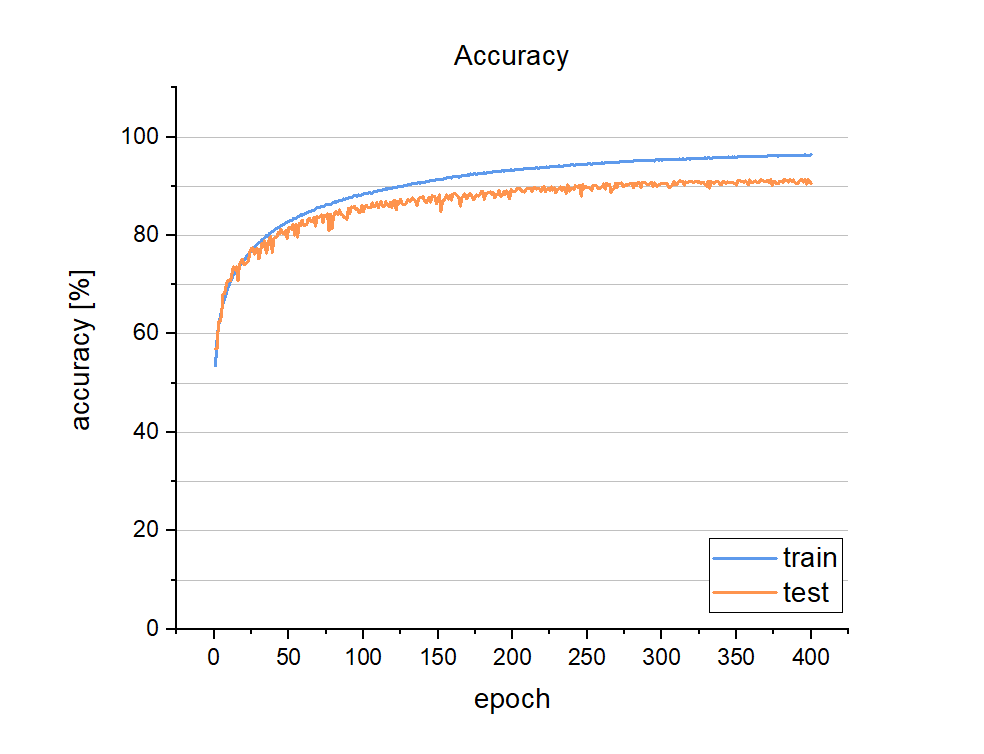
\includegraphics[width=\linewidth]{resources/accuracy.PNG}
        \captionsetup{width=\linewidth}
        \captionof{figure}{Accuracy of presented model}
        \label{fig:accuracy}
    \end{minipage}%
    \begin{minipage}{.5\textwidth}
        \centering
        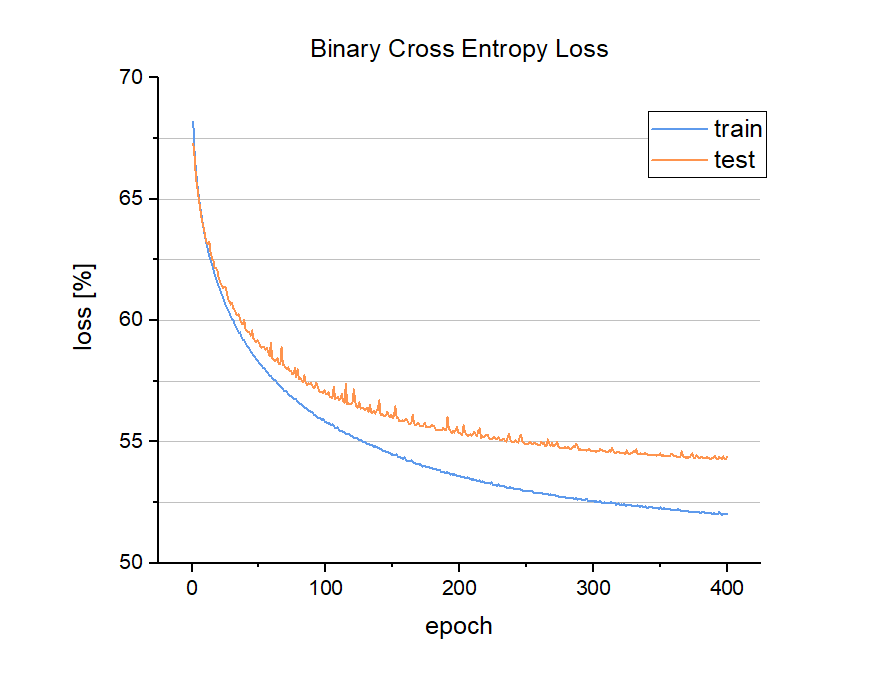
\includegraphics[width=\linewidth]{resources/loss.PNG}
        \captionsetup{width=\linewidth}
        \captionof{figure}{Value of loss function used in model}
        \label{fig:loss}
    \end{minipage}
\end{figure}

The results presented in \mbox{Tab.~\ref{tab:confusion-matrix}} show that the model provides correct prediction, most of the samples are classified to an appropriate category.
The value of \gls{far} is relatively acceptable; however, the \gls{frr} is significantly higher than in commercial applications.

Chong et al.~\cite{Main} present a similar approach to the related problem and in many cases, they achieved very low values of \gls{frr} and \gls{far}.
In this work, using \gls{cnn}'s as a core of a solution, a little bit poorer results were achieved.
The authors of this study consider the small dataset as the main foundation of this behavior and despite the data augmentation and other applied techniques, the results did not reach the values from the cited work.
